\chapter{Asistente web interactivo para la simplificación de textos}
\label{cap:asistente}

	\chapterquote{La tecnología hace posible lo que antes era imposible. El diseño hace que sea real}{Michael Gagliano}

En este capítulo hablamos sobre el proceso de diseño de la aplicación o web, las dificultades que nos hemos ido encontrando en su desarrollo, los cambios que ha ido sufriendo y las mejoras hasta llegar a su versión final.

Nuestro asistente tiene como su principal finalidad la adaptación de textos, que puedan suponer un grado mayor de esfuerzo por parte del lector, convirtiéndolo en Lectura Fácil.

Para ello, la herramienta consta de las siguientes funcionalidades:
\begin{itemize}
\item Resumen del texto introducido.
\item Identificación de palabras complejas en el texto.
\item Intercambio de orden de palabras o conjunto de palabras.
\item Listado de sinónimos de una palabra. Contaremos con sinónimos tanto complejos como otros más sencillos.
\item Listado de definiciones de una palabra.
\item Eliminación de una o varias palabras.
\end{itemize}
\section{Arquitectura}\label{sec:arquitectura}

Hemos usado una arquitectura REST basada en endpoints, por la cual el frontend en html puro y javascript hara llamadas a los endpoints del backend para todo aquello que suponga una operación de carga lógica o de llamada a terceros, como la API de NILWS o funciones que requieran la libreria de Spacy.

También decidimos esta arquitectura por la posibilidad original de usar una base de datos para el almacenaje de información del uso que le daría un usuario, como que palabra es la mas cambiada, y su posible futuro uso para predicción. Sin embargo, esto a quedado como trabajo a futuro, pero la posibilidad esta abierta con la estructura actual.

En la sección  \ref{sec:backend} se describe el Back End y en la sección \ref{sec:frontend} el Front End.

\section{Back End}\label{sec:backend}

El Back End se encarga de toda la lógica necesarias para que la web funcione correctamente, siendo estos transparentes al usuario. Se trata de una serie de procesos o funciones no podemos ver.

Está desarrollado con Flask usando Python como lenguaje, implementando con esto una arquitectura REST basada en endpoints.
REST es una arquitectura de desarrollo web que puede ser utilizada en cualquier cliente HTTP y se basa en cuatro operaciones básicas: GET, POST, PUT y DELETE.
\begin{itemize}
	\item \textbf{GET} se utiliza para acceder a los distintos recursos. Si requiere del envío de un parámetro al servidor, este se pasa como un elemento en la URI. Si se necesitara pasar mas de un elemento, tendría que hacerse mediante una petición POST
	
	\item \textbf{POST} se utiliza para realizar acciones de creación de nuevos recursos. Si se requiere el envío de información al servidor, esta se pasa dentro del cuerpo de la petición HTTP.
	
	\item \textbf{PUT} se utiliza para la modificación de los recursos existentes. Como con la operación POST, la información se envía dentro del cuerpo de la petición HTTP
	
	\item \textbf{DELETE} se utiliza para eliminar los recursos. Como con GET, la información va por la URI.
\end{itemize}
Las llamadas a estas operaciones se implementan como peticiones HTTP, con la URI del recurso, con respuesta del servidor. Estas respuestas serán un código de estado como 200 OK, 404 NOT FOUND, etc...

Todos los endpoints definen la URI y tipo de operación con la etiqueta  @app.route y devuelven un objeto en formato JSON.

\begin{itemize}
	\item \textbf{simple} \label{isSimple}: En este endpoint recibimos una lista de objetos JSON, cada uno con un id y una palabra, que en su conjunto forman la frase de la cual queremos resaltar las palabras complejas.
	\begin{lstlisting}[language=Python]
		@app.route('/isSimple', methods=['POST'])
		def simple():
		data=request.get_json()
		data=data['text']
		nlp=spacy.load("es_core_news_sm")
		textList=[]
		for word in data:
		textList.append(word['text'])
		text=' '.join(textList)
		doc=nlp(text)
		position=0
		simpleList=[]
		simple=False
		for token in doc:
		pos=token.pos_
		if (pos != "ADP" and pos != "DET"
		and pos != "CONJ" and pos != "NUM"
		and pos != "PRON" and pos != "PUNCT"
		and pos != "SCONJ" and pos != "SYM"
		and pos != "X" and pos!="SPACE"):
		simple=isSimple(unidecode(token.text))
		else:
		simple=None
		simpleList.append({'id':data[position]['id'],'simple':simple})
		position+=1
		jsonList=json.dumps(simpleList)
		return jsonify(simpleList=jsonList)
	\end{lstlisting}
	A partir de cada palabra contenida en la lista original formamos la frase y la convertimos en un objeto de Spacy, el cual nos da las anotaciones lingüísticas de cada palabra del texto, de las cuales en este caso usaremos el etiquetado gramatical de cada palabra para filtrar aquellas que no sean sencillas o complejas, como los signos de puntuación o los símbolos.
	Si se pasa el filtro, se hará una llamada a la API de NILWS, previamente mencionada en el capítulo \ref{cap:herramientas} sección \ref{sec:nilws}
	Hecho esto se devolverá al frontend una lista de objetos los cuales tienen cada uno un id y un boolean que identifique si es sencilla o no.
	
	\item \textbf{definition}\label{definition}: Dada una palabra, este endpoint devolverá su definición.
	\begin{lstlisting}[language=Python]
		@app.route('/definition', methods=['POST'])
		def definition():
		word=request.get_json()
		word=word['word']
		response = requests.get(NILWS_URL + word + DEFINITION_URL)
		data = response.json()
		d=data['definiciones']
		return jsonify(definiciones=data['definiciones'])
	\end{lstlisting}
	Para conocer la definición de la palabra se hace una llamada al endpoint de definiciones de NILWS.
	
	\item \textbf{summary}\label{summary}: Este endpoint devolverá un resumen de un texto dado. Este resumen esta hecho dando importancia a las frases del texto según el numero de veces que aparece una palabra en la frase. Después se devolverán el 40\% de las frases que hemos considerado mas importantes.
	\begin{lstlisting}[language=Python]
		@app.route('/summary', methods=['POST'])
		def sentenceSummary():
		data = request.get_json()
		text = data["text"]
		nlp = spacy.load("es_core_news_sm")
		docx = nlp(text)
		allWords = [word.text for word in docx]
		extraWords = list(STOP_WORDS) + list(punctuation) + ['\n']
		freqWord = {}
		for word in allWords:
		aux = word.lower()
		if aux not in extraWords and aux.isalpha():
		if aux in freqWord.keys():
		freqWord[aux] += 1
		else:
		freqWord[aux] = 1
		val=sorted(freqWord.values())
		maxFreq=val[-3:]
		for word in freqWord.keys():
		freqWord[word] = (freqWord[word]/maxFreq[-1])
		sentStrength={}
		for sent in docx.sents:
		for word in sent :
		if word.text.lower() in freqWord.keys():
		if sent in sentStrength.keys():
		sentStrength[sent]+=freqWord[word.text.lower()]
		else:
		sentStrength[sent]=freqWord[word.text.lower()]
		else:
		continue
		topSentences = (sorted(sentStrength.values())[::-1])
		top40percentSent = int(0.4*len(topSentences))
		topSent = topSentences[:top40percentSent]
		summary = []
		for sent,strength in sentStrength.items():
		if strength in topSent:
		summary.append(sent.text)
		else:
		continue
		return jsonify(summary=summary)
	\end{lstlisting}
	Convertimos el texto original en un objeto de Spacy y para cada palabra guardamos en un array su frecuencia de aparición.
	Asignamos a cada frase una importancia segun las palabras mas frecuentes del texto y devolvemos el 40\% de ellas.
	
	\item \textbf{sentenceTree} \label{sentencesTree}: Dada una frase generamos su arbol de dependencias usando Spacy.
	\begin{lstlisting}[language=Python]
		@app.route('/sentences/tree', methods=['POST'])
		def sentenceTree():
		data = request.get_json()
		sentence = data["sentence"]
		nlp = spacy.load("es_core_news_sm")
		doc = nlp(sentence)
		jsonTree = ''
		sentenceIds = []
		for sent in doc.sents:
		tree = to_nltk_tree(sent.root, 0)
		for word in sent:
		sentenceIds.append({'text': word.text, 'id': word.i})
		jsonTree = jsonify(tree=tree.serialize(), sentenceIds=sentenceIds)
		return jsonTree
	\end{lstlisting}
	Generamos el objeto Spacy y recorremos todas su frases, que en este caso siempre sera una, generamos el árbol a partir de la palabra que Spacy ha identificado como la raíz de la cual dependen el resto de palabras. 
	Devolveremos el árbol en un formato JSON y una lista que contenga la palabra y el id que le hemos asignado, el cual es la posición original de la palabra en la frase.
	
	\item \textbf{sentences} \label{sentences}: Dado un texto, este endpoint devolverá las frases que lo componen.
	\begin{lstlisting}[language=Python]
		@app.route('/sentences', methods=['POST'])
		def splitTextInSentences():
		data = request.get_json()
		text = data["text"]
		sentences = []
		nlp = spacy.load("es_core_news_sm")
		doc = nlp(text)
		for sent in doc.sents:
		sentences.append(sent.text)
		return jsonify(sentences=sentences)
	\end{lstlisting}
	Generamos un objeto Spacy a partir del texto, el cual identifica automáticamente las frases de las que esta compuesto, y devolvemos una lista de las frases.
	
	\item \textbf{synonymous} \label{synonymous}: A partir de una palabra generamos los sinónimos que tenga y los dividimos en sencillos y complejos.
	\begin{lstlisting}[language=Python]
		@app.route('/synonymous', methods=['POST'])
		def synonymous():
		data = request.get_json()
		synonymous = unidecode(data["synonymous"])
		response = requests.get(NILWS_URL + synonymous + SYNONYMOUS_URL)
		synosymousASCII = response.json()
		completeSynonymousList = synosymousASCII['sinonimos']
		simpleSynonymousList = []
		synonymousList = []
		for token in completeSynonymousList:
		word = token['sinonimo']
		if isSimple(word):
		simpleSynonymousList.append(word)
		else:
		synonymousList.append(word)
		return jsonify(synonymous=synonymousList, 
		simpleSynonymous=simpleSynonymousList)	
	\end{lstlisting}
	Hacemos una petición a la API de NILWS de la palabra recibida, a la que previamente le quitamos todos los caracteres especiales, ya que la petición es tipo GET y no admite este tipo de caracteres en la URI de la llamada.
	Dada la lista de sinónimos de la palabra, comprobamos si es simple o no haciendo otra petición a la misma API y devolvemos la lista de los sinónimos sencillos y la de los complejos.
	
\end{itemize}



\section{Front End}\label{sec:frontend}

Para el desarrollo del Front End nuestro asistente hará uso del lenguaje HTML, CSS para definir los estilos (colores, tamaños, disposición, fuentes...) en lo que se refiere a la parte visual. Hemos utilizado el lenguaje Javascript para interaccionar con la parte del Back End, siendo así indispensable para ejecutar los diferentes eventos y funcionalidades.
 
 



 
%Para el desarrollo de esta parte, detallamos brevemente tres lenguajes que son esenciales: 


 
%\begin{itemize}
%	\item \textbf{HTML}: son las siglas en inglés \textit{HyperText Markup Lenguage} que significa lenguaje de marcado de etiquetas, una herramienta de elaboración de páginas web. Se trata de un conjunto de etiquetas que sirven para definir el texto y otros elementos que compondrán la página como imágenes, listas, vídeos, etc. Los ficheros HTML, tienen una extensión ``.html''. 
%	
%	\item \textbf{CSS}: son las siglas en inglés \textit{Cascading Style Sheets} que significa hoja de estilos en cascada, que sirve para aplicar estilos (colores, tamaños, alineación, tipo de fuente...) a un fichero HTML (páginas web). Los ficheros CSS, tienen una extensión ``.css''.
%	
%		\item \textbf{JavaScript}: es un lenguaje de programación interpretado, no es necesario compilarlo para ejecutarlo, que se usa para crear páginas web dinámicas. Incorpora efectos, acciones a ejecutar, animaciones, cambio de estilo, etc., que permite la interactividad con el usuario. Se ejecuta siempre en la parte del cliente. Los ficheros JavaScript, tienen una extensión ``.js''.
%	
%\end{itemize}
\subsection{Desarrollo de las interfaces del asistente Lectura Fácil}

En la Figura \ref{fig:interfazInicial} se observa la interfaz inicial de nuestro asistente: 
\begin{figure}[h!]
	\centering
	
	
	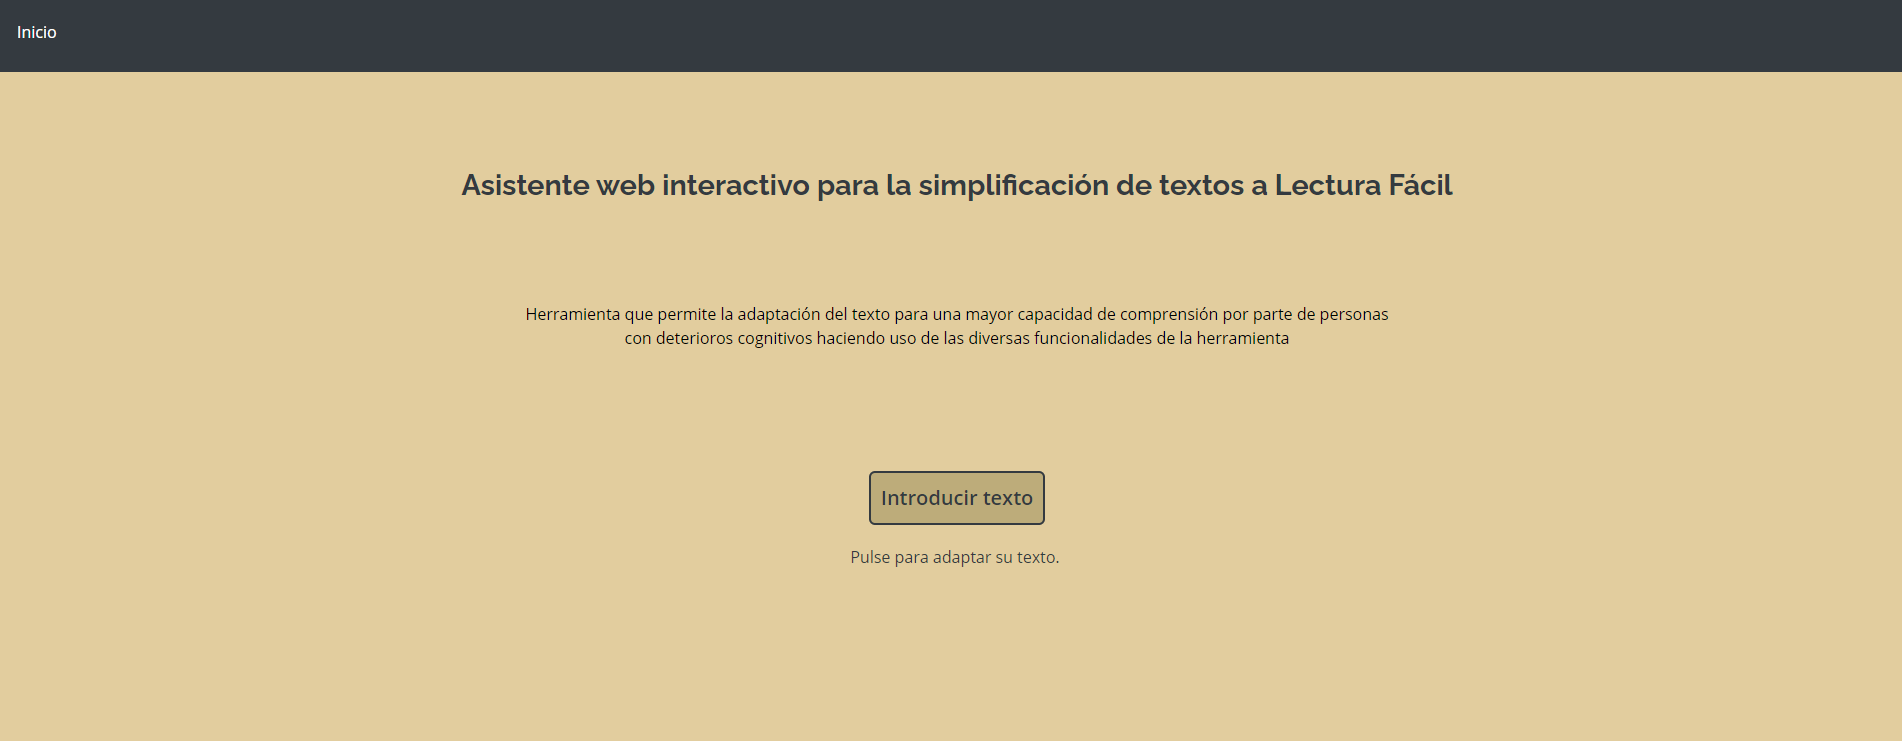
\includegraphics[scale=0.4]{Imagenes/Figuras/InterfazInicial}


\caption{Interfaz inicial del asistente.}
\label{fig:interfazInicial}
\end{figure}


Cuando el usuario haga click en ``Introducir texto'', se le mostrará un nuevo panel para que lo introduzca. De esta manera, podrá elegir entre resumirlo o continuar con el texto original.


En la Figura \ref{fig:interfazIntroduccionTexto} se muestra la interfaz que observaría el usuario:

\begin{figure}[h!]
	\centering
	
	
	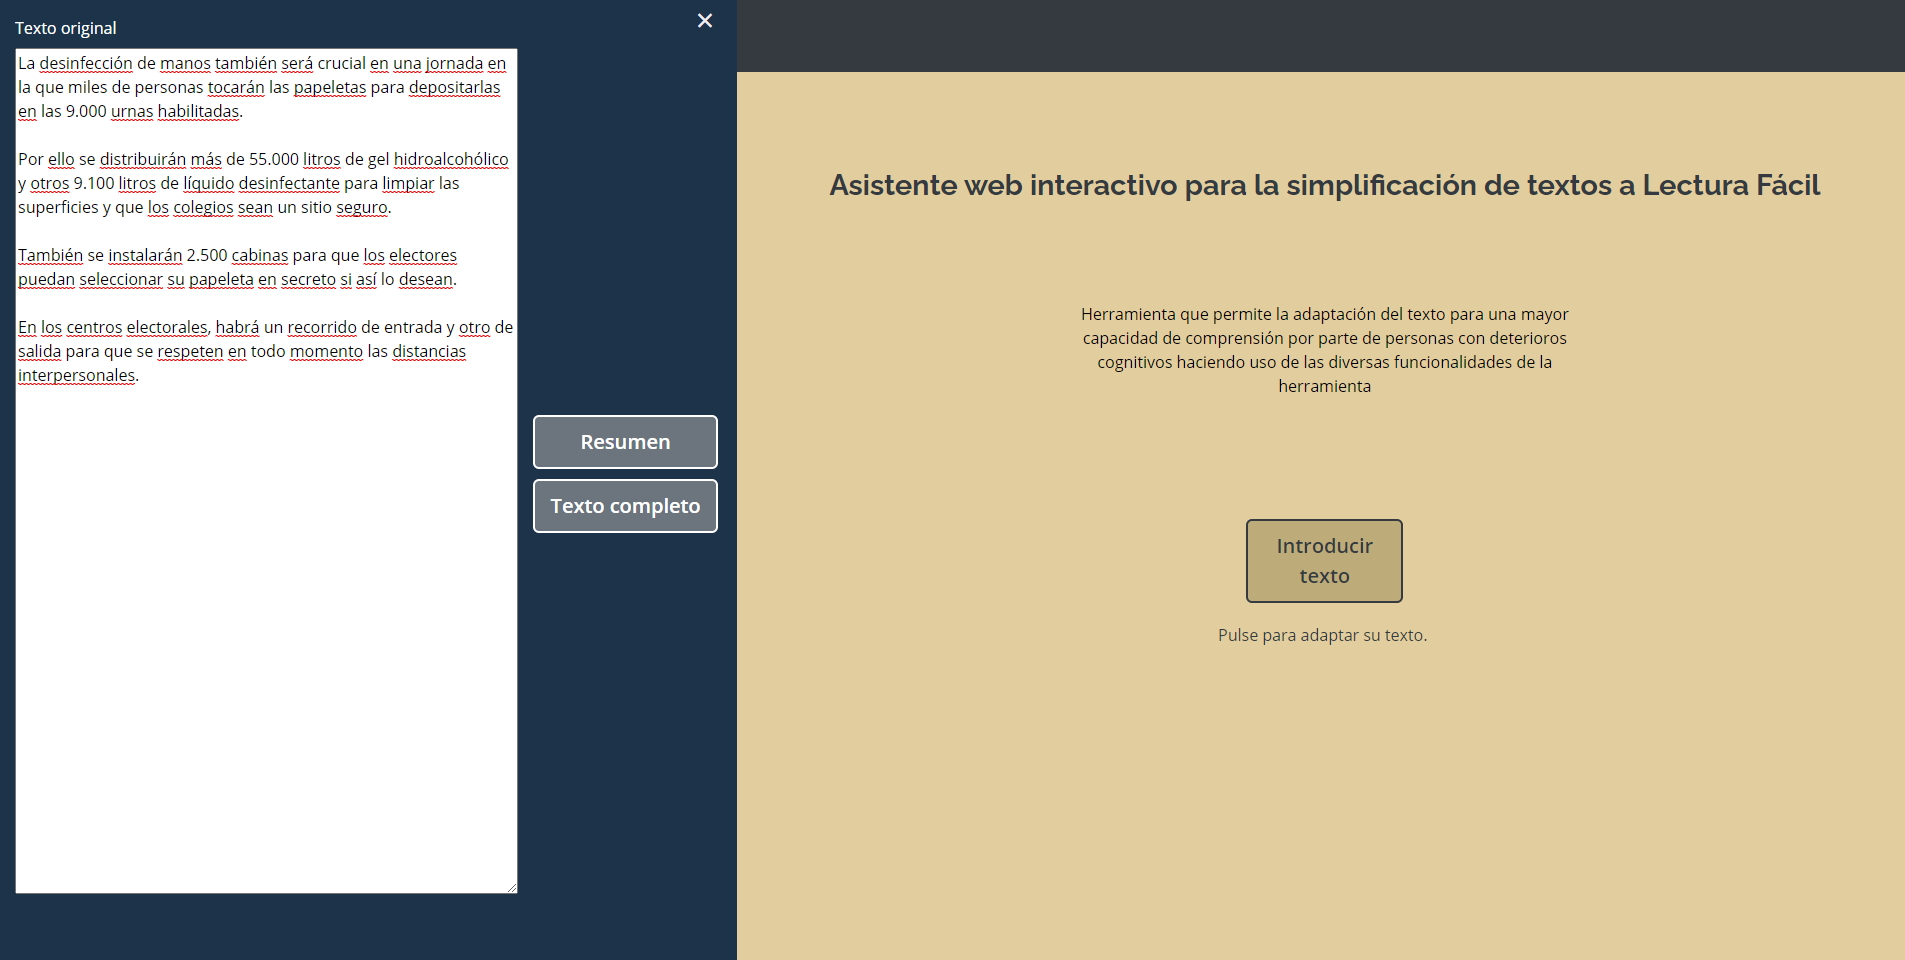
\includegraphics[scale=0.4]{Imagenes/Figuras/InterfazPanelIntroducirTexto}


\caption{Introducción de texto.}
\label{fig:interfazIntroduccionTexto}
\end{figure}

	
A continuación, una vez se seleccione bien ``Resumen'' (Figura \ref{fig:interfazFraseTextoResumido}), bien ``Texto completo'' (Figura \ref{fig:interfazIntroducirCompleto}), se muestra una serie de frases seleccionables partiendo de un texto resumido o completo (ver sección \ref{summary} del Back End). 


\begin{figure}[h!]
	\centering
	
	
	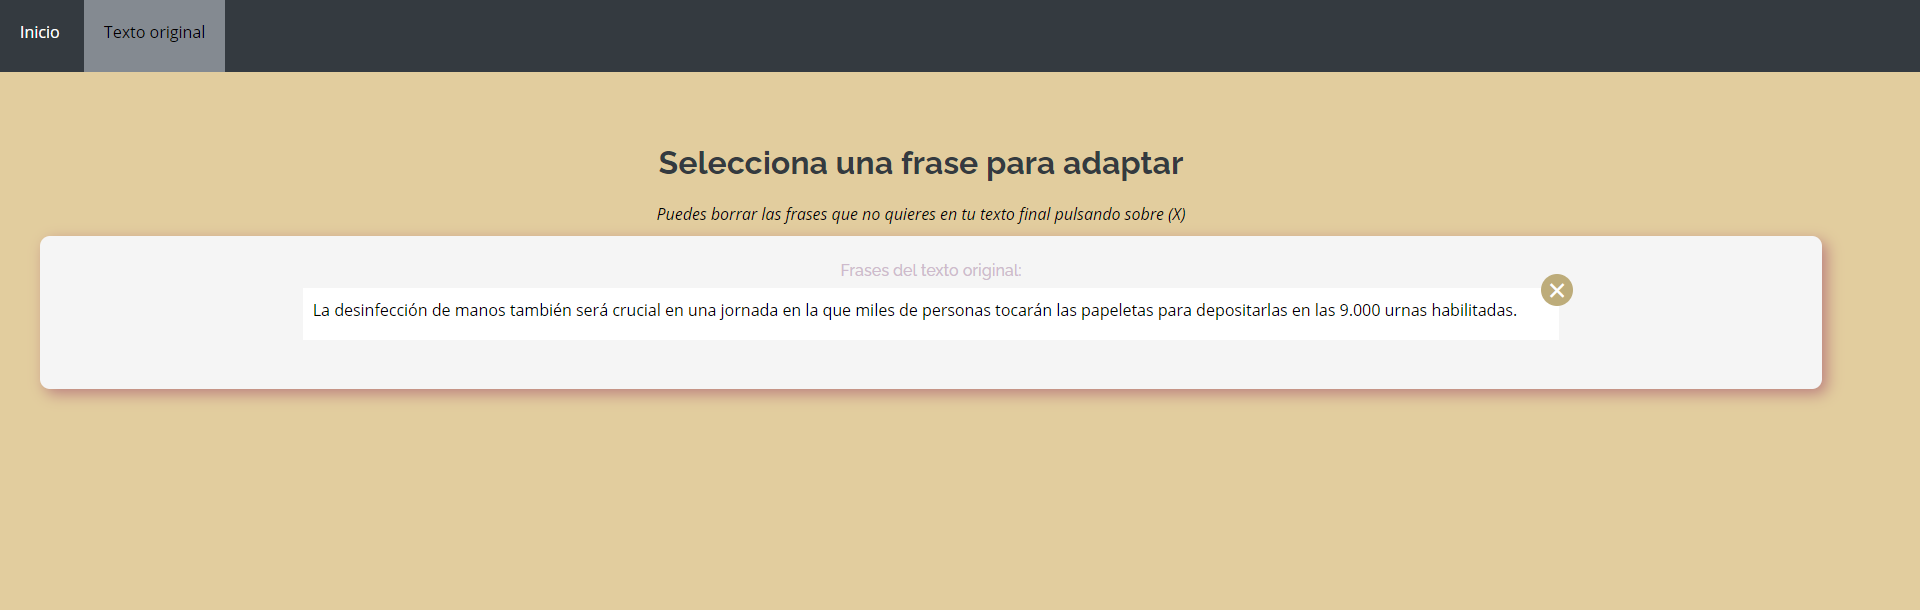
\includegraphics[scale=0.4]{Imagenes/Figuras/FrasesTextoResumido}
	
	
	\caption{Selección de frase con texto resumido.}
	\label{fig:interfazFraseTextoResumido}
\end{figure}


\begin{figure}[h!]
	\centering
	
	
	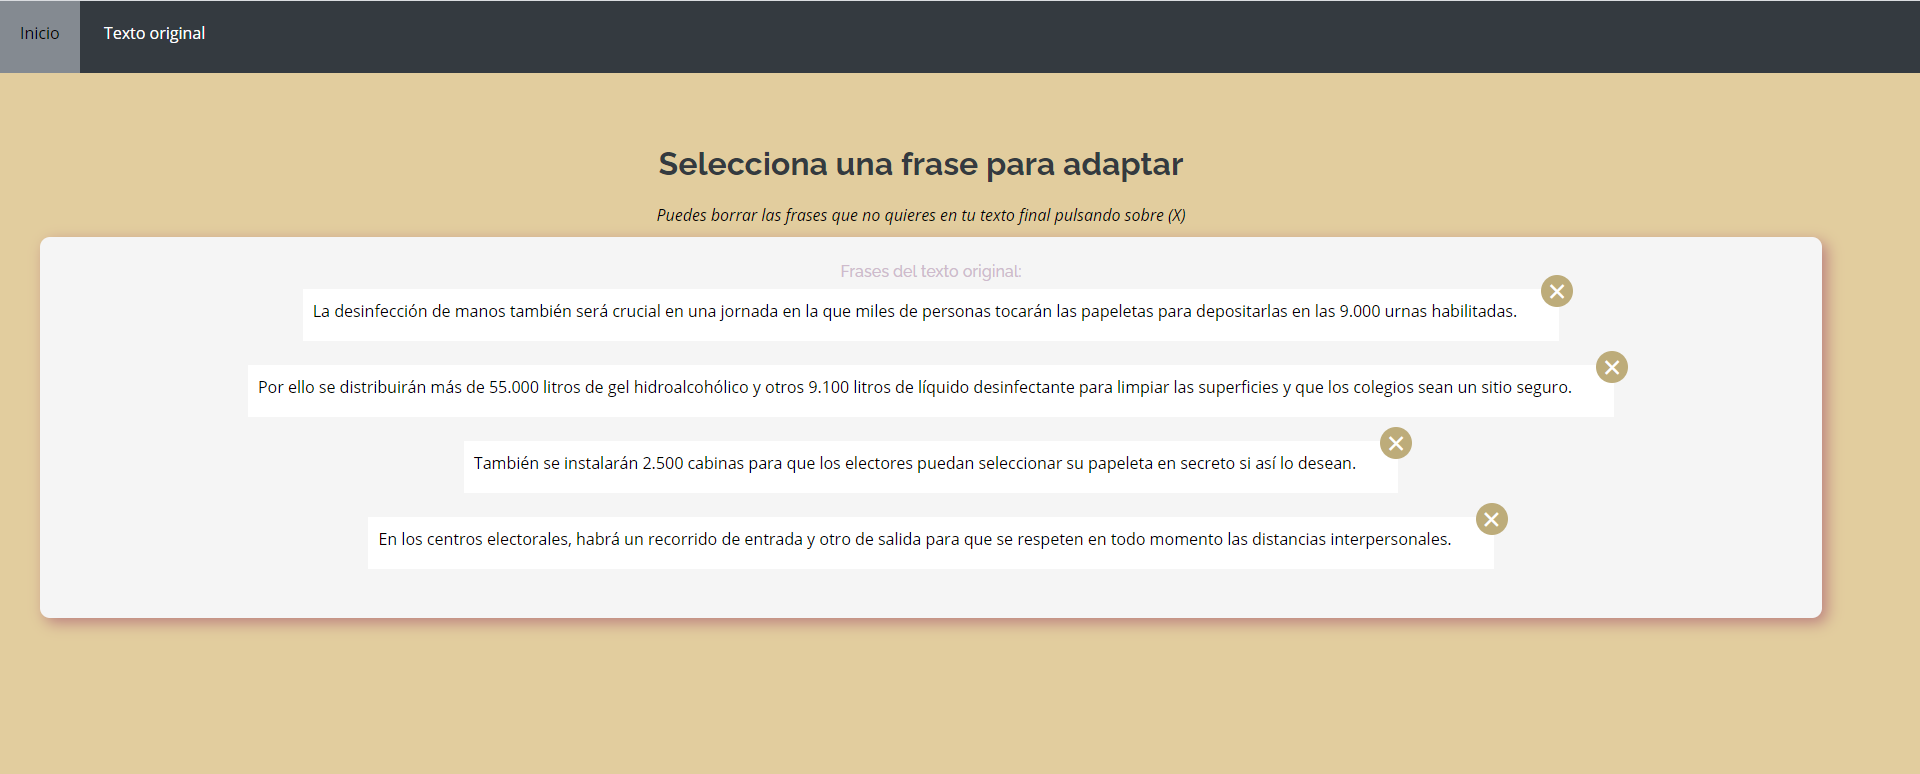
\includegraphics[scale=0.4]{Imagenes/Figuras/FrasesTextoCompleto}
	
	
	\caption{Selección de frase con texto original.}
	\label{fig:interfazIntroducirCompleto}
\end{figure}


En la siguiente interfaz (Figura \ref{fig:interfazArbolFuncionalidades}) podemos observar que ya se nos permite hacer uso de diferentes funcionalidades para adaptar nuestro texto, teniendo el árbol de dependencias un papel vital a la hora de hacer posible esta adaptación de una forma interactiva.
\begin{figure}[H]
	\centering
	
	
	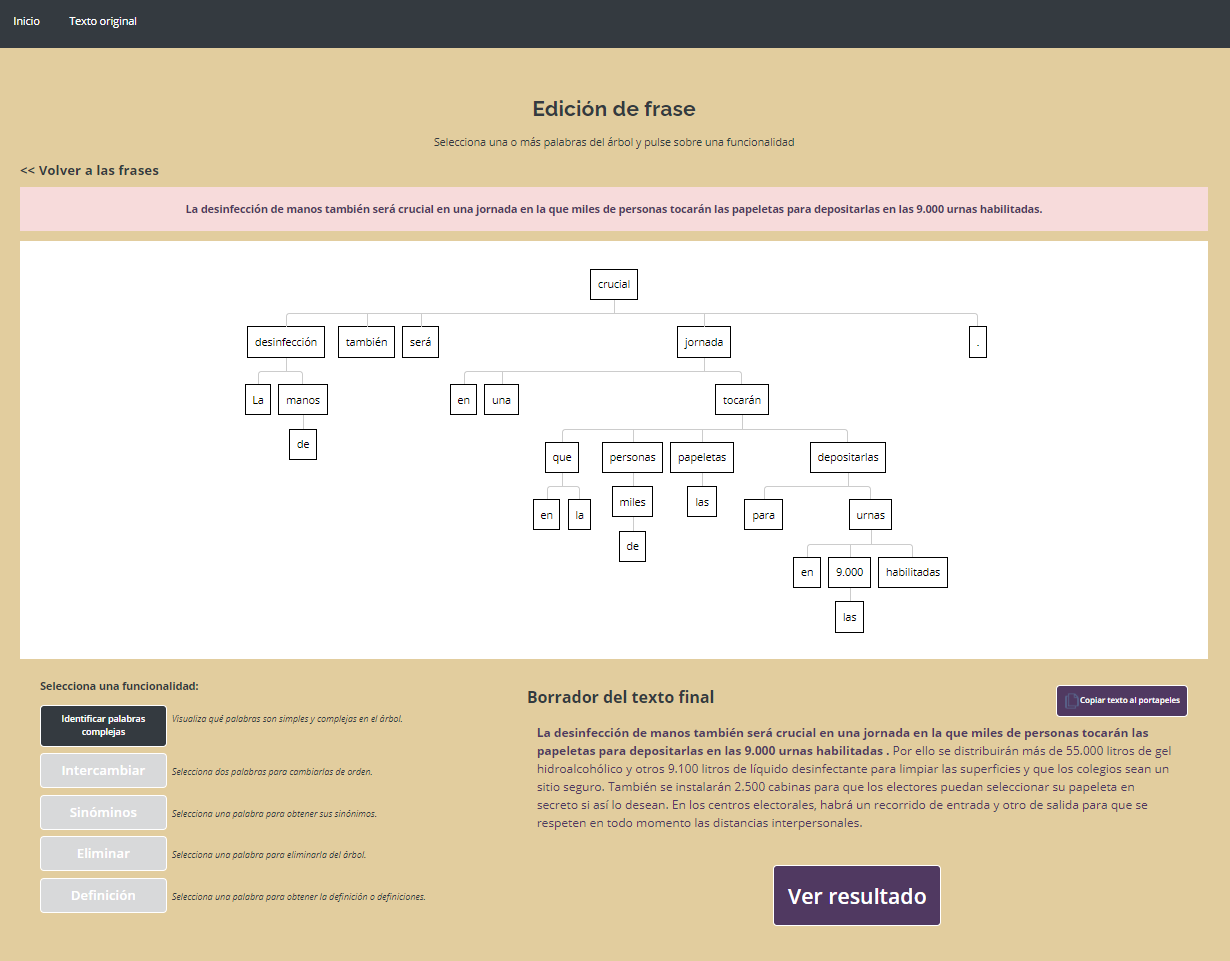
\includegraphics[scale=0.6]{Imagenes/Figuras/ArbolYFuncionalidades}
	
	
	\caption{Interfaz para adaptar texto.}
	\label{fig:interfazArbolFuncionalidades}
\end{figure}


\subsubsection{Árbol de dependencias}
	El árbol de dependencias se construye mediante una función llamada ``buildTree()'' que se basa en un algoritmo de búsqueda en profundidad (BFS), recorriendo todos los nodos (en nuestro caso palabras de la frase) de un árbol mediante un objeto JSON recibido de la parte Back End, que podemos ver con más detalle en la sección \ref{sentencesTree}. El funcionamiento de este algoritmo consiste en ir expandiendo cada uno de sus nodos desde la raíz hacia el nodo hoja (no tiene más hijos) de manera recurrente (Figura \ref{fig:algoritmoBFS}).
	
		\begin{figure}[h!]
		\centering
		
		
		\subfloat{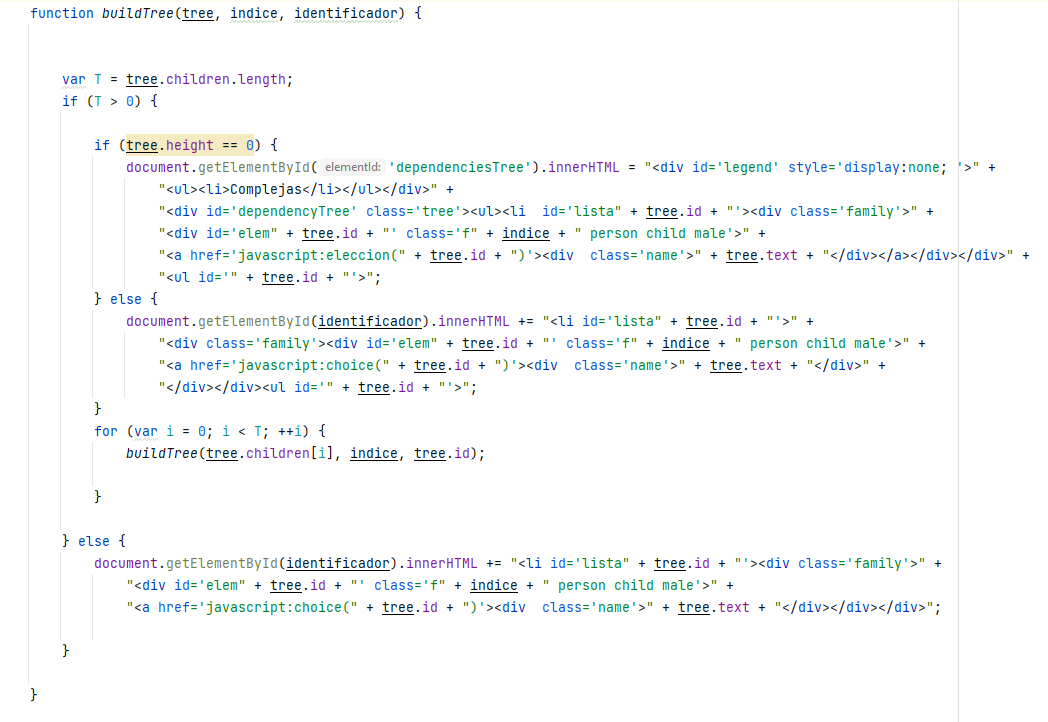
\includegraphics[scale=0.5]{Imagenes/Figuras/algoritmoBFS}}
		
		
		\caption{Código del algoritmo BFS.}
		\label{fig:algoritmoBFS}
	\end{figure}

	Por ejemplo, supongamos que queramos adaptar la frase ``También se instalarán 2.500 cabinas para que los electores puedan seleccionar su papeleta en secreto si así lo desean.'', el objeto JSON tendría el aspecto de la Figura \ref{fig:objetoJSON}. 
	Cada nodo contiene los siguientes datos:
	\begin{itemize}
		\item \textbf{children}: array de nodos hijos.
		\item \textbf{height}: nivel del nodo con respecto a la raíz (en nuestro ejemplo ``instalarán'' sería nuestra raíz, que tiene una altura 0).
		\item \textbf{id}: identificador único de cada nodo.
		\item \textbf{text}: palabra propia del nodo.
	\end{itemize}

		\begin{figure}[h!]
		\centering
		
		
		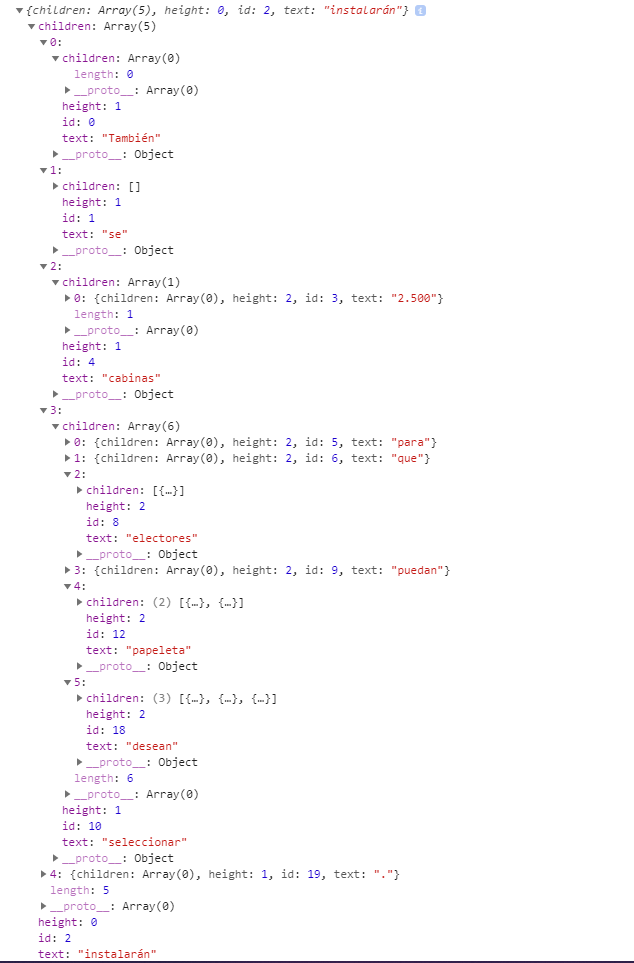
\includegraphics[scale=0.5]{Imagenes/Figuras/ObjetoArbolEjemplo}
		
		
		\caption{Objeto JSON.}
		\label{fig:objetoJSON}
	\end{figure}

En la Figura \ref{fig:arbolDependencias} observamos el árbol con el que podremos interactuar durante la adaptación.
	
		\begin{figure}[h!]
		\centering
		
		
		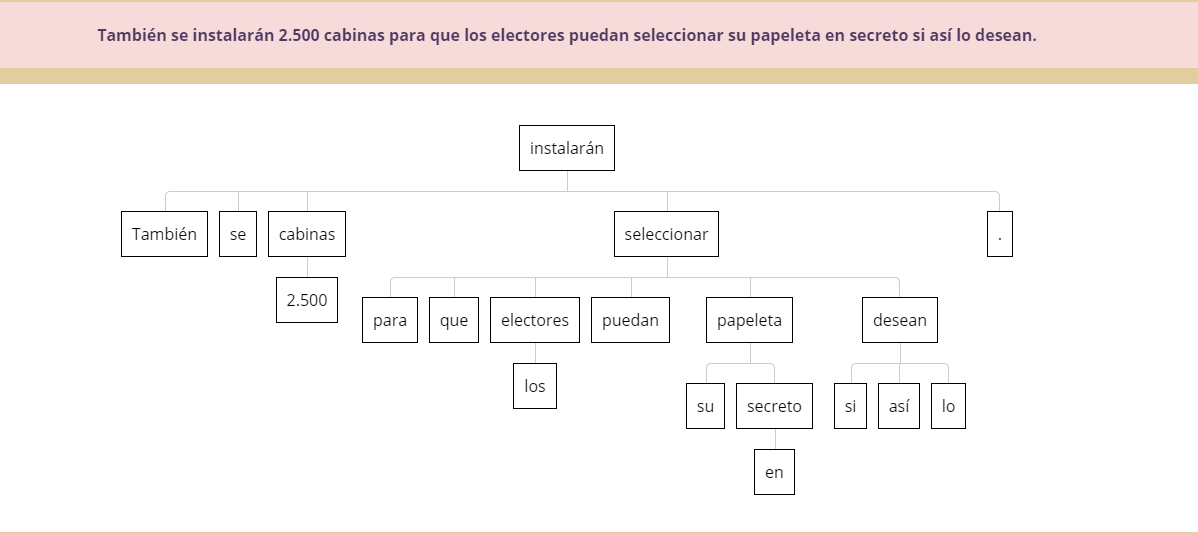
\includegraphics[scale=0.6]{Imagenes/Figuras/ArbolEjemploObjeto}
		
		
		\caption{Árbol de dependencias.}
		\label{fig:arbolDependencias}
	\end{figure}
	

	\subsubsection{Funcionalidades de adaptación}






Las diferentes funcionalidades que nos ofrece el asistente para adaptar nuestro texto a Lectura Fácil son:

\begin{itemize}
	\item \textbf{Identificar palabras complejas}: permite mostrar en nuestro árbol de dependencias las palabras complejas o que puedan tener más dificultad de comprensión. 
	
	En esta funcionalidad recibimos de la parte de Back (ver sección \ref{isSimple} del Back End) un objeto, que se muestra en la Figura \ref{fig:InterfazActivarPalabrasComplejas}.
		 \begin{figure}[h!]
			\centering
			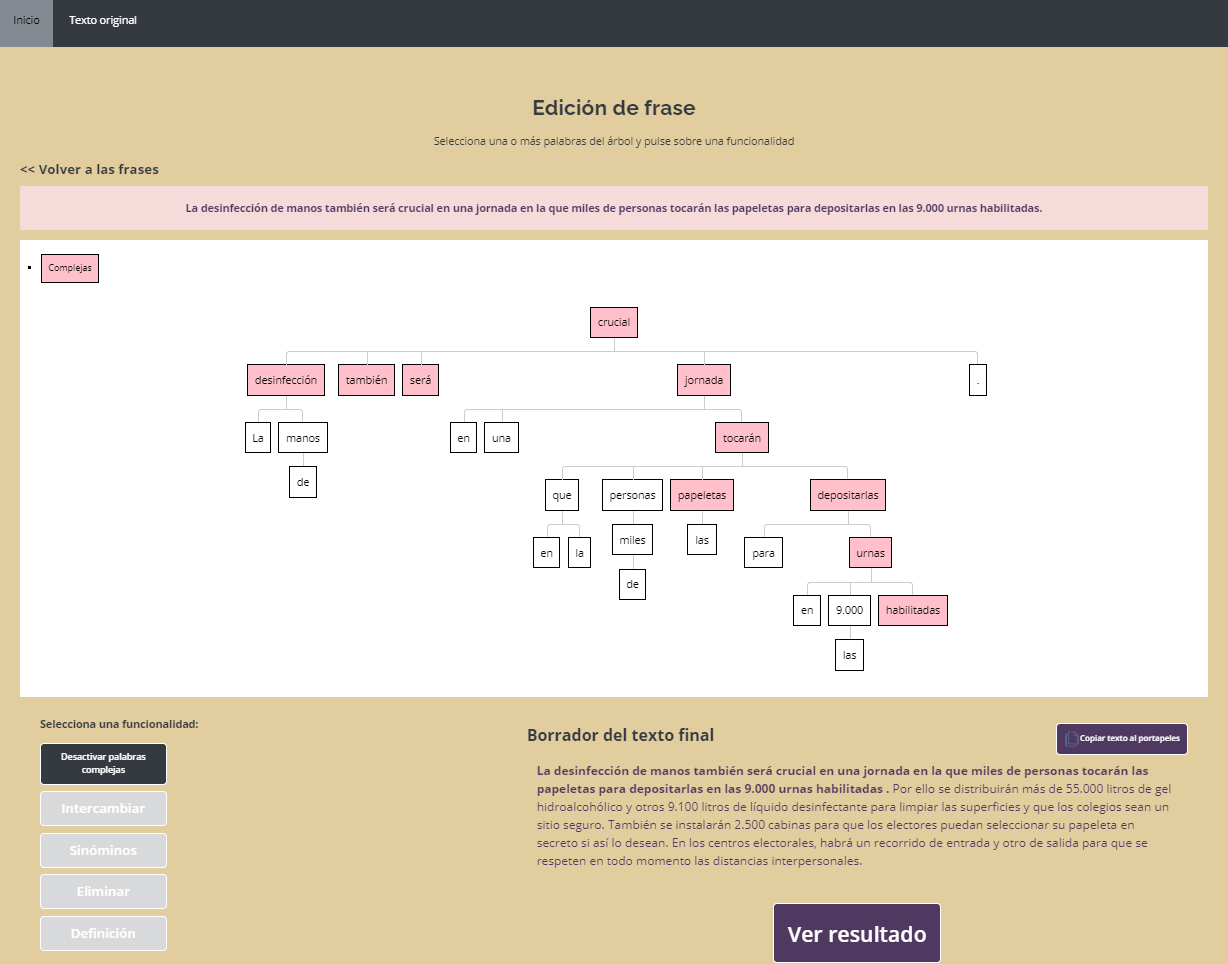
\includegraphics[scale=0.6]{Imagenes/Figuras/ActivarPalabrasComplejas}
			
			\caption{Interfaz para observar palabras complejas en el árbol.}
			\label{fig:InterfazActivarPalabrasComplejas}
		\end{figure}
		Cada nodo contiene los siguientes datos:
		
	\begin{itemize}
		\item \textbf{id}: identificador único de cada nodo.
		\item \textbf{simple}: booleano con valor ``False'' si la palabra es compleja.
  


	\end{itemize}
En la interfaz veremos una leyenda indicando el color con el que se muestran estas palabras complejas.

	\item \textbf{Desactivar palabras complejas}: vuelve a la vista original del árbol de dependencias sin resaltar las palabras complejas. 

   \item \textbf{Intercambiar}: seleccionadas dos palabras del árbol, cambiamos las posiciones de ambas incluyendo las palabras que dependan de ellas.
   Durante el desarrollo de esta parte hemos tratado la funcionalidad de dos maneras diferentes tanto para modificar el árbol como para el borrador del texto final:
\begin{itemize}
   \item Si las dos palabras son padre e hijo, se intercambia solo las palabras sin modificar otros nodos dependientes de ellos. En este caso, para escribir en el borrador la frase resultante (marcada en negrita), se intercambian sus ids. 
   \item Si el caso anterior no se da, se intercambia ambos nodos incluyendo los nodos dependientes. En este caso, para escribir en el borrador la frase resultante, se guarda en un array los ids involucrados, es decir, aquellos que formen parte de las palabras seleccionadas en el intercambio incluyendo estas, ordenándolos de menor a mayor, para saber la posición inicial de dichos nodos. A continuación, se forma una sublista con los nodos de la primera palabra seleccionada (Figura \ref{fig:intercambio}\subref{fig:intercambioPaso1}). Una vez eliminada esta sublista del array original (Figura \ref{fig:intercambio}\subref{fig:intercambioPaso2}), se evalúa la nueva posición en la que se encuentra la segunda sublista (Figura \ref{fig:intercambio}\subref{fig:intercambioPaso3}) y se vuelve a eliminar del array de partida (Figura \ref{fig:intercambio}\subref{fig:intercambioPaso4}). Por último se inserta la segunda sublista en la posición de la primera y viceversa(Figura \ref{fig:intercambio}\subref{fig:intercambioPaso5}), teniendo así nuestra frase con este intercambio (Figura \ref{fig:resultadoIntercambio}).

\begin{figure}[H]
	\begin{center}
		\subfigure[Creación de la primera sublista del array original]{
			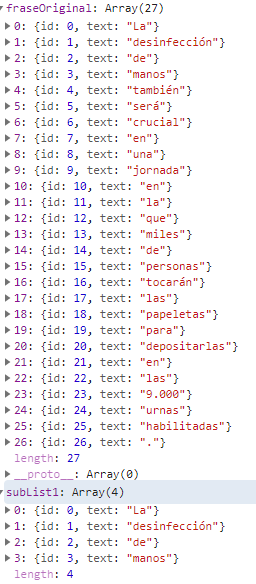
\includegraphics[width=0.3\textwidth]{Imagenes/Figuras/IntercambioPaso1}
	\label{fig:intercambioPaso1}}
		\subfigure[Extracción de la primera sublista en el array original]{
			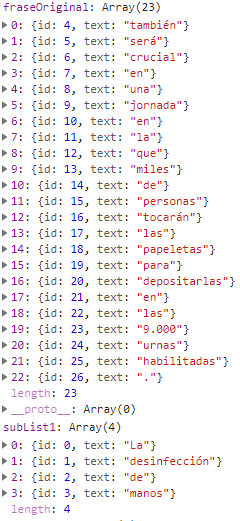
\includegraphics[width=0.3\textwidth]{Imagenes/Figuras/IntercambioPaso1_2}
		\label{fig:intercambioPaso2}}
		\subfigure[Creación de la segunda sublista del array original]{
			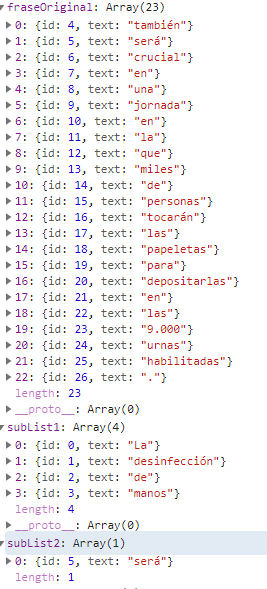
\includegraphics[width=0.3\textwidth]{Imagenes/Figuras/IntercambioPaso2_1}
		\label{fig:intercambioPaso3}}
		\subfigure[Extracción de la segunda sublista del array original]{
			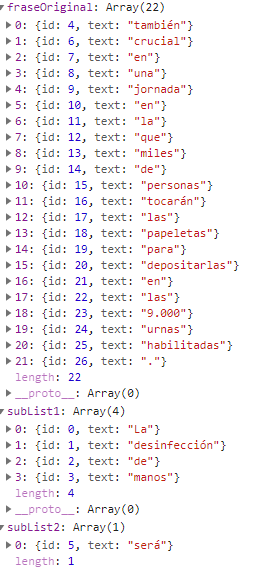
\includegraphics[width=0.3\textwidth]{Imagenes/Figuras/Intercambio2_2}
		\label{fig:intercambioPaso4}}
		\subfigure[Inserción de ambas sublistas en el array original]{
			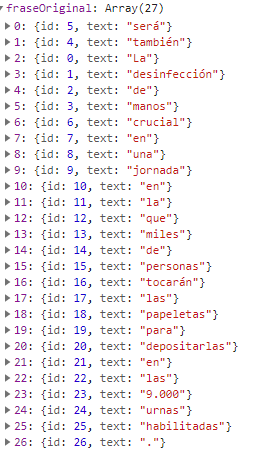
\includegraphics[width=0.3\textwidth]{Imagenes/Figuras/Intercambio3}
		\label{fig:intercambioPaso5}}
		\caption{Pasos del intercambio de palabras.}
		\label{fig:intercambio}
	\end{center}
\end{figure}
   

	 \begin{figure}[h!]
	\centering
	
	
	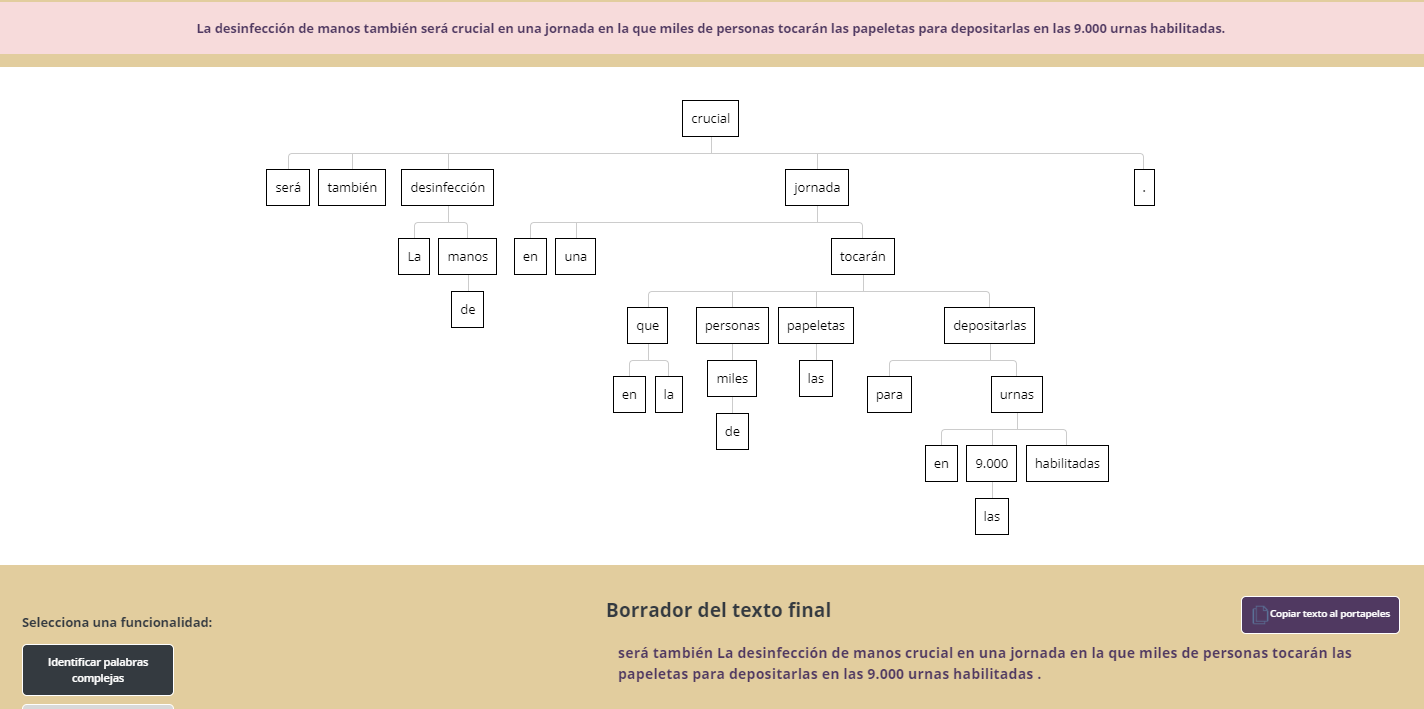
\includegraphics[scale=0.5]{Imagenes/Figuras/IntercambioResultante}
	
	
	\caption{Interfaz resultante de intercambiar dos palabras.}
	\label{fig:resultadoIntercambio}
\end{figure}
\end{itemize}


\item \textbf{Sinónimos}: una vez seleccionemos una palabra del árbol, se nos mostrará un listado de otras palabras que puedan ser más sencillas o complejas que posean el mismo significado (Figura \ref{fig:listaSinonimos}). Podemos hacer referencia a la sección  \ref{synonymous} del Back End. En esta funcionalidad puede darse el inconveniente de que no concuerde correctamente el sinónimo cambiado, en número, persona o conjugación con el contexto de la frase. Para solucionarlo, hemos optado por que el usuario pueda ser capaz de editarlo in situ (véase la Figura \ref{fig:edicionSinonimos}).
	 \begin{figure}[h!]
	\centering
	
	
	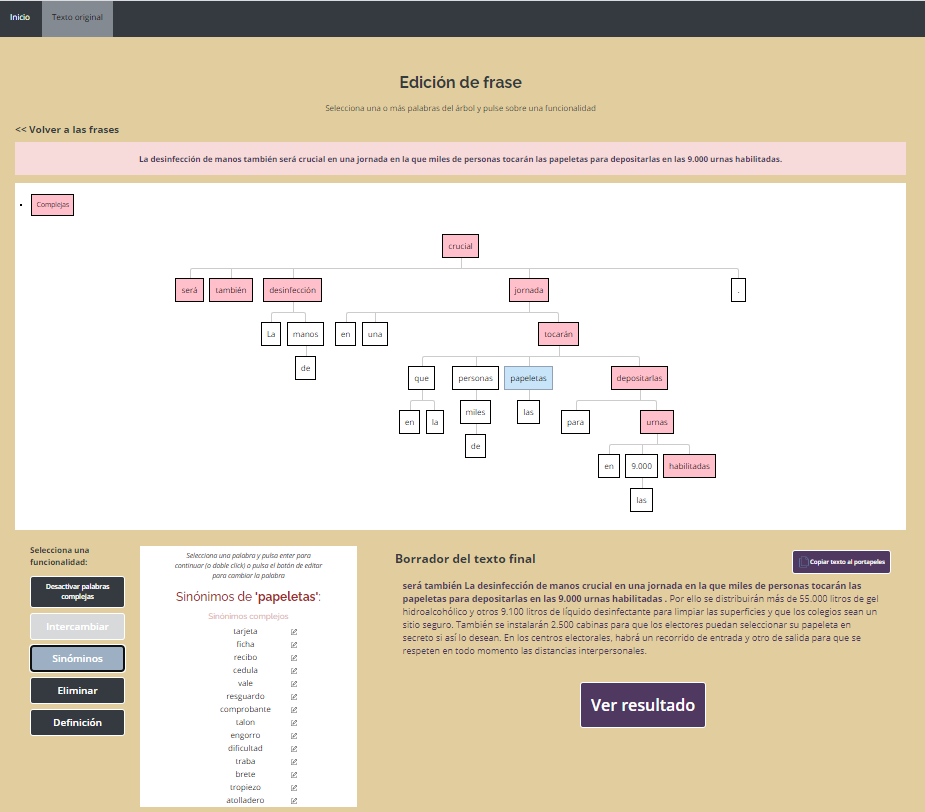
\includegraphics[scale=0.56]{Imagenes/Figuras/SinonimosComplejos}
	
	
	\caption{Interfaz con la lista de sinónimos de una palabra seleccionada}
	\label{fig:listaSinonimos}
\end{figure}
	 \begin{figure}[h!]
	\centering
	
	
	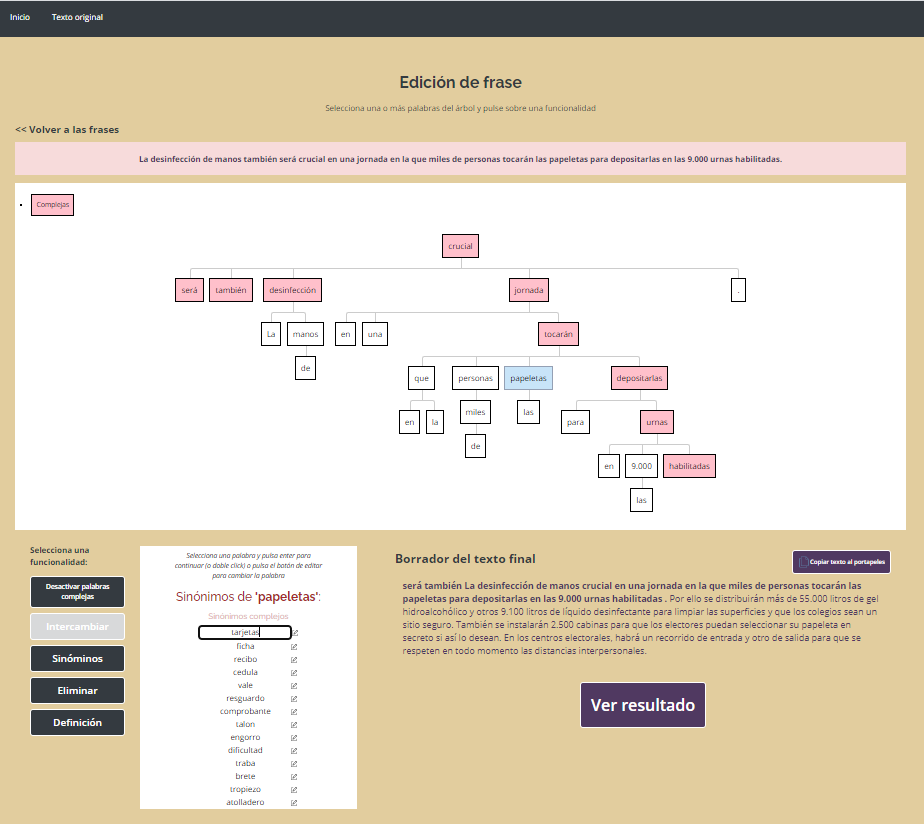
\includegraphics[scale=0.6]{Imagenes/Figuras/EdicionSinonimos}
	
	
	\caption{Interfaz de edición de sinónimos}
	\label{fig:edicionSinonimos}
\end{figure}



Vemos en la Figura \ref{fig:resultadoSinonimos} cómo quedaría el árbol y la frase resultante del borrador una vez utilizado esta parte funcional.
	 \begin{figure}[h!]
	\centering
	
	
	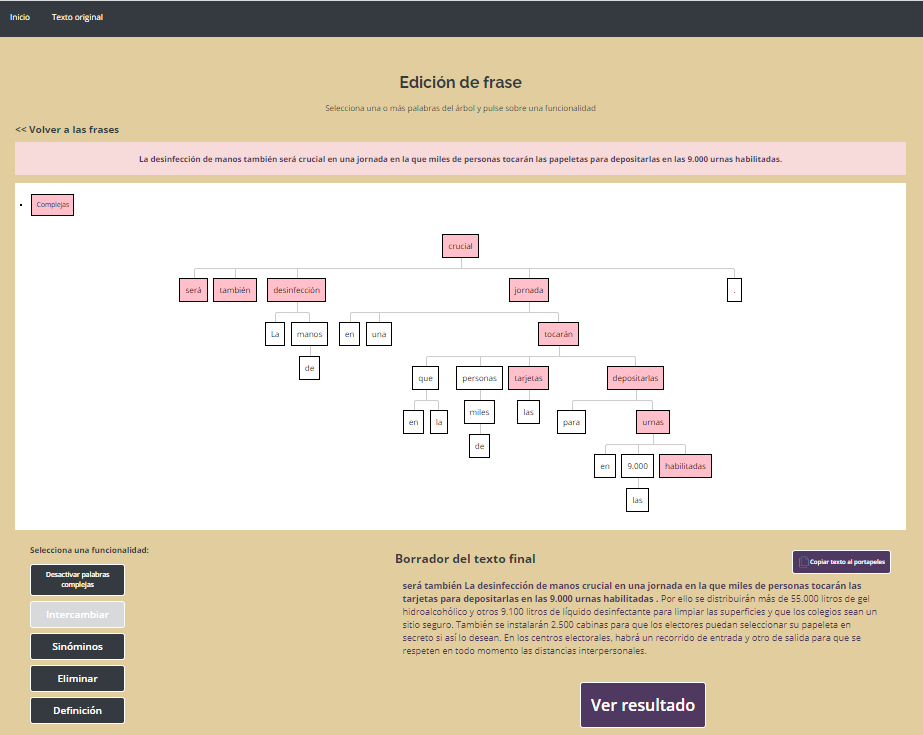
\includegraphics[scale=0.57]{Imagenes/Figuras/ResultadoSinonimos}
	
	
	\caption{Interfaz una vez cambiado la palabra por un sinónimo}
	\label{fig:resultadoSinonimos}
\end{figure}

\item \textbf{Eliminar}: seleccionada una palabra de nuestro árbol, borra tanto a ella como aquellas que dependan de ella. Partiendo del objeto JSON recibido a la hora de construir el árbol, hacemos uso de un array auxiliar donde recogemos los ids de la/s palabras a eliminar y se extraen del array original, eliminando así las palabras de la frase original (Figura \ref{fig:eliminacion}, se elimina la palabra ``urnas'' y sus dependientes).
	 \begin{figure}[h!]
	\centering
	
	
	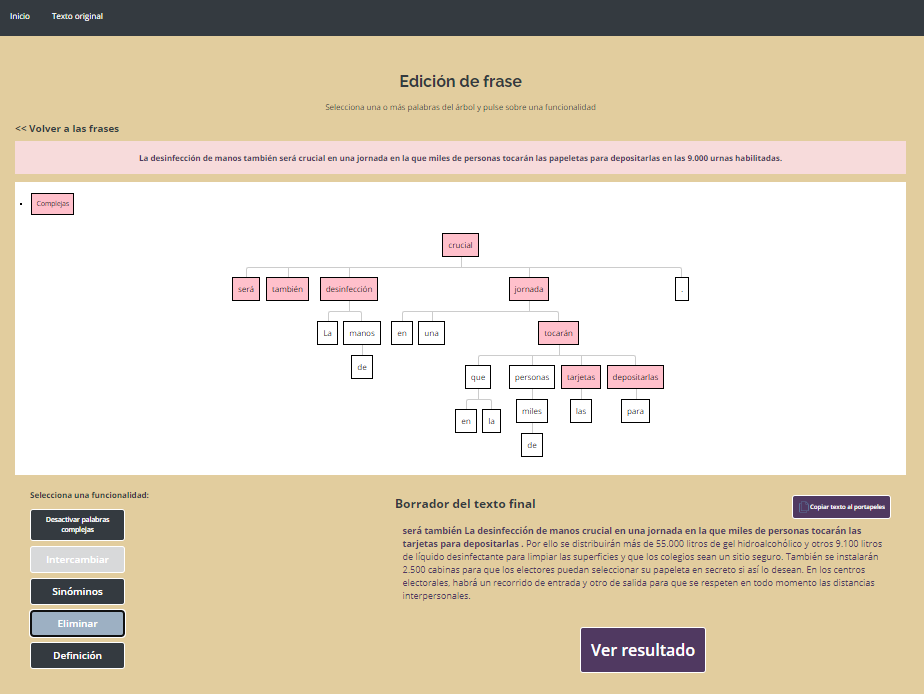
\includegraphics[scale=0.56]{Imagenes/Figuras/EliminacionNodos}
	
	
	\caption{Interfaz tras la eliminación}
	\label{fig:eliminacion}
\end{figure} 

\item \textbf{Definición}: dado un término seleccionado en el árbol, podemos obtener su glosario de manera que podamos escoger una o varias definiciones y adjuntarlas como parte del texto final, que sirva de apoyo a la comprensión del mismo (Figura \ref{fig:definiciones}). Ver sección \ref{definition} de Back End.
	 \begin{figure}[h!]
	\centering
	
	
	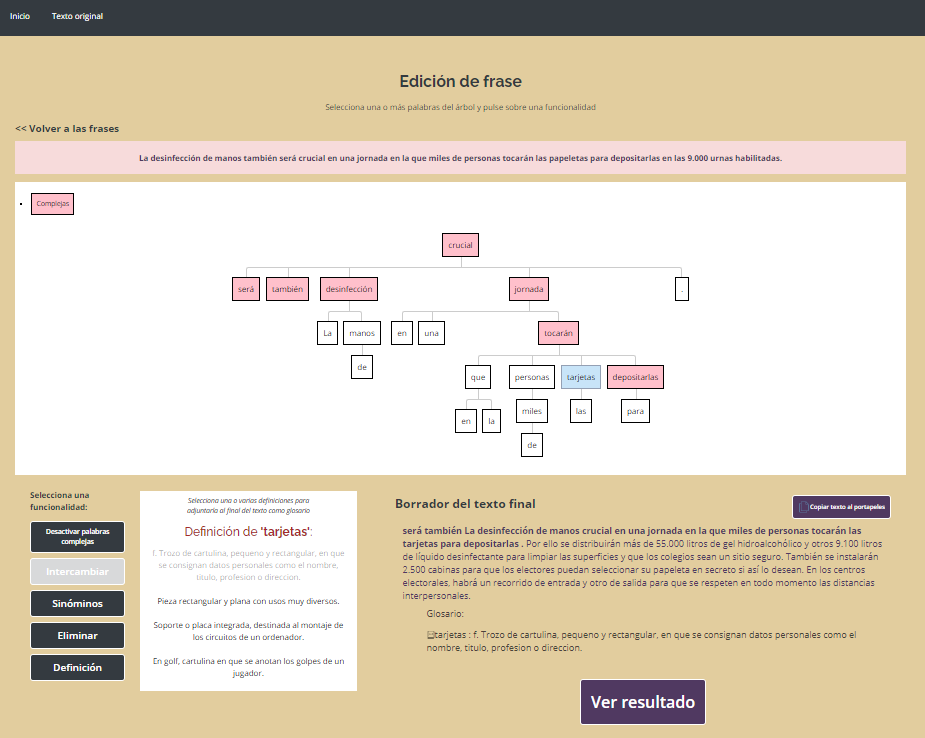
\includegraphics[scale=0.55]{Imagenes/Figuras/definiciones}
	
	
	\caption{Interfaz con el listado de las definiciones}
	\label{fig:definiciones}
\end{figure}
\end{itemize}

   
   
   
%   \begin{figure}[h]
%   	\centering
%   	
%   	
%   	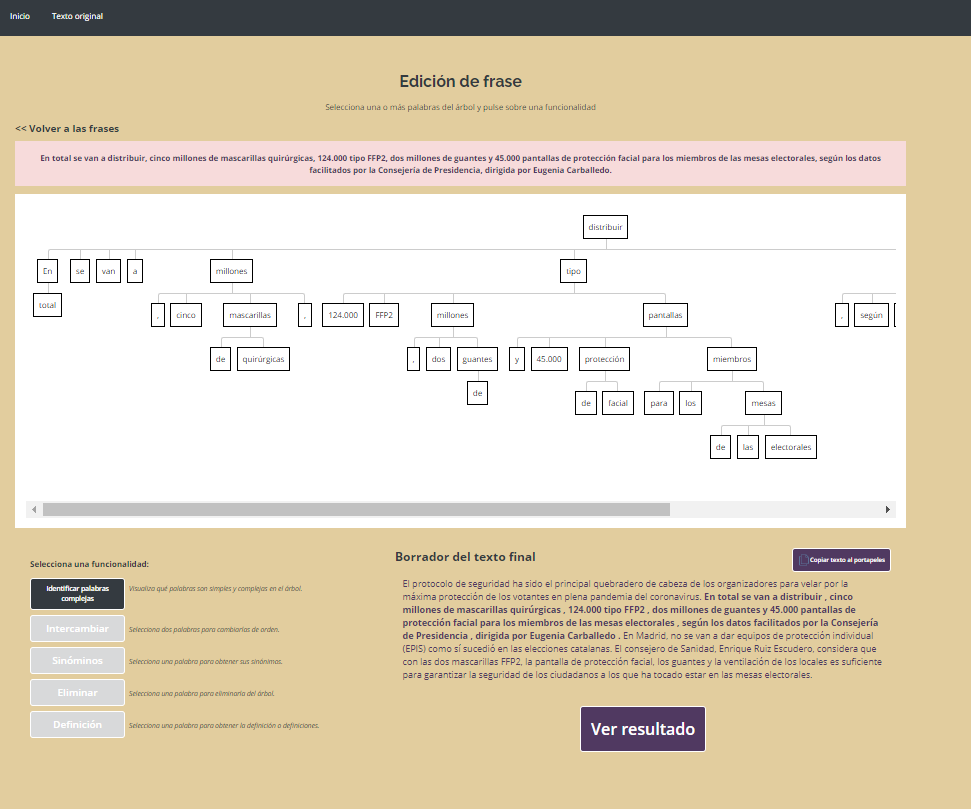
\includegraphics[width=1.0\textwidth]{Imagenes/Figuras/InterfazArbolFuncionalidades}
%   	
%   	
%   	\caption{Interfaz sin las palabras complejas resaltadas}
%   	\label{fig:interfazArbolFuncionalidades}
%   \end{figure}



\subsubsection{Resultado de la adaptación}

Una vez ya consideremos que nuestro texto esté adaptado a nuestras necesidades, podemos visualizarlo en la siguiente interfaz una vez el usuario haya clicado en "Ver resultado" (Figura \ref{fig:resultadoFinal}). Cabe destacar que el panel en donde aparece el texto final, es editable. Esto es útil, por ejemplo, en el caso de que las frases se quieran cambiar de orden entre sí.
	 \begin{figure}[h!]
	\centering
	
	
	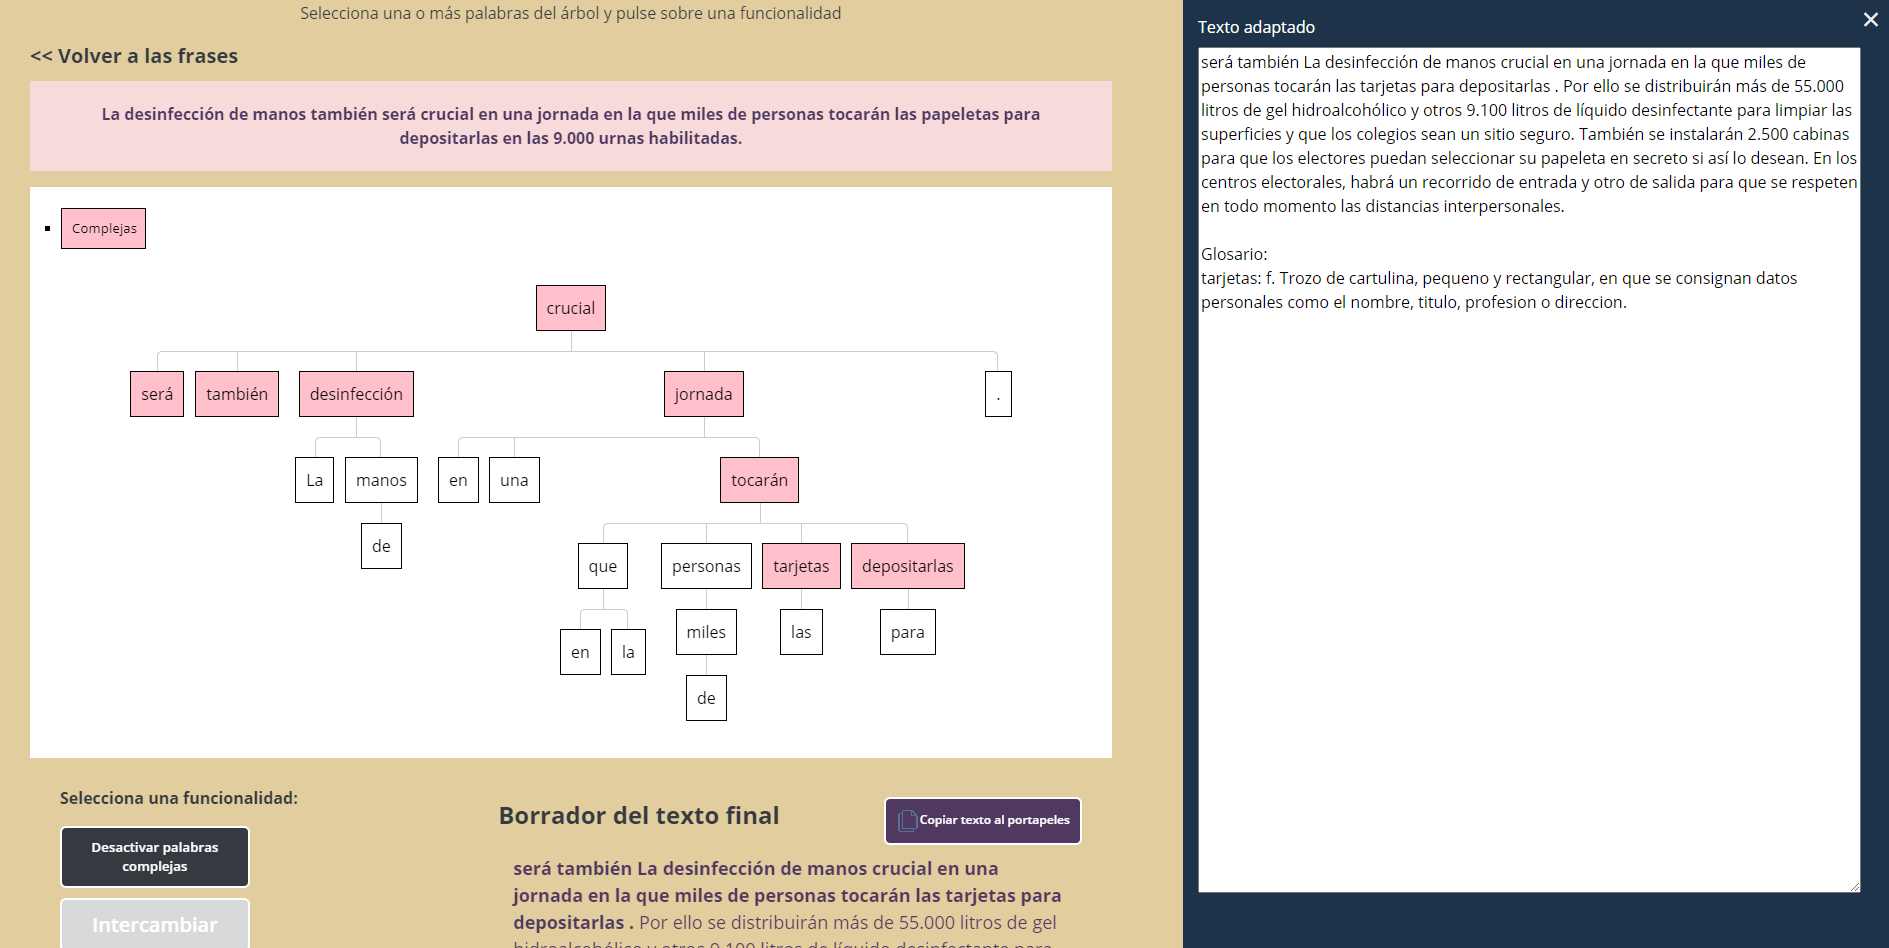
\includegraphics[scale=0.3]{Imagenes/Figuras/ResultadoFinal}
	
	
	\caption{Interfaz del resultado final con el texto adaptado}
	\label{fig:resultadoFinal}
\end{figure}


Además, el botón ``Copiar al portapapeles'' nos da la opción de copiar el texto del borrador para poder introducirlo en cualquier herramienta externa.


 